\chapter{Methodik}
Im Abschnitt \ref{sec:variational_autoencoder} wurde bereits die Funktionsweise und das Optimieren des VAE Modells beschrieben. Im folgenden wird erklärt, wie neue Beispiele generiert werden. Außerdem werden Details zu den Modellarchitekturen gezeigt.



\section{Latent-Space Sampling}\label{sec:sampling}
Der Variational Autoencoder besitzt einen strukturierten Latent-Space. Daher kann zwischen den Erwartungswerten $\mu_1 = \mu_\phi(x_1)$ und $\mu_2 = \mu_\phi(x_2)$ vom Encoder berechneten Normalverteilung interpoliert werden. Es werden im Folgenden vier verschiedene Sampling Methoden vorgestellt, um neue Latent-Vektoren $\hat{z}$ zu erzeugen. Diese wurden in leicht anderer Form von \cite{Jorge2018} vorgeschlagen. Die erste Methode ist aus der Standardnormalverteilung $\cN(0, 1)$ zu sampeln. Dies ist sinnvoll, da der Encoder durch den KL-Term dazu gezwungen ist, nicht zu sehr von $\cN(0, 1)$ abzuweichen. Eine weitere Methode ist, den Erwartungswert eines original Beispiels $\mu_\phi(x)$, welcher das Zentrum der dazugehörigen Normalverteilung repräsentiert, zu modifizieren. Betrachtet werden drei Modifikationen: Addieren von Gauss-Rauschen (Noise), Interpolation und Extrapolation. Für die Noise Variante wird zufälliges Rauschen einer Normalverteilung $\cN(0, \alpha)$ auf den Eingabe- Erwartungswert addiert.
\begin{equation}\label{eq:add_noise}
  \hat{z_i} = z_i + \epsilon, \epsilon \sim \cN(0, \alpha)
\end{equation}
Für die Wahl Interpolations Partner wird eine $k$-Nächster-Nachbar Suche im Latent-Space durchgeführt. Gesucht wird unter allen Erwartungswerten $\mu_\phi(x_i)$ für Eingaben $x_i$. $\hat{z}_i$ repräsentiert den modifizierten Latent-Vektor. Das Vorzeichen vor $\alpha$ bestimmt, ob interpoliert oder extrapoliert wird. $\alpha$ ist ein zu setzender Hyperparameter und definiert die Stärke der Inter-/Extrapolation
\begin{equation}
  \hat{z_i} = \pm \alpha \cdot \left[\mu_\phi(x_k) - \mu_\phi(x_i)\right] + \mu_\phi(x_i)
\end{equation}



\section{Single-VAE}
Dieses Verfahren trainiert ein VAE Modell auf dem gesamten Datensatz. Das Training erfolgt selbst-überwacht, d.h. es werden keine Informationen über die Klassen benötigt. Vorteil dieses Ansatzes ist, dass große Datenmengen genutzt werden können, welche nicht annotiert sein müssen. Es erschwert allerdings das Sampling neuer Beispiele, denn für einen Latent-Vektor $\hat{z}_i$ ist nicht definiert, welcher Klasse er angehört. Der Single-VAE wird deshalb nur mit den Sampling Methoden Noise, Interpolation und Extrapolation für die Data Augmentation genutzt. Das Originalbeispiel, welches für Generation modifiziert wird, definiert dabei die Klasse des generierten Beispiels. Weitere Ansätze, wie das Nutzen eines Klassifikators, welcher die Klasse zu $\hat{z}_i$ bestimmt, wurden nicht weiter verfolgt.



\section{Multi-VAE}\label{sec:multi-vae-intro}
Ein von \cite{Moreno-Barea2020} angeführtes Problem mit dem Single-VAE Ansatz besteht darin, dass ein einzelner VAE bei imbalancierten Datensätzen dazu tendiert, die größere Klasse im Latent-Space zu überrepräsentieren. Um dem entgegen zu wirken, schlagen die Autoren vor, nur einen VAE pro Klasse zu trainieren. Dazu werden die Daten in $k$ Submengen aufgeteilt, wobei $k$ die Anzahl der verschiedenen Klassen bezeichnet. Jede dieser $k$ Klassen besteht aus den der Klasse zugehörigen Daten. Außerdem wird eine Variante untersucht, bei der zusätzlich noch zufällige Beispiele der anderen Klassen mit einem Anteil von 20\% hinzugefügt werden (Bezeichnet mit "Mix Data"). Falls Klassen bestimmte Merkmale teilen, kann dies dem Encoder helfen, diese zu extrahieren. Die Abbildung \ref{fig:dataset_parts} veranschaulicht die Aufteilung des Datensatzes. Das Training der einzelnen VAEs erfolgt auf den klassenweisen Datensätzen. Neue Beispiele können somit leicht über Sampling aus einer Standard Normalverteilung generiert werden. Die Klasse des neuen Beispiels ist die zugehörige Klasse des VAEs.

\begin{figure}[hbt]
  \centering
  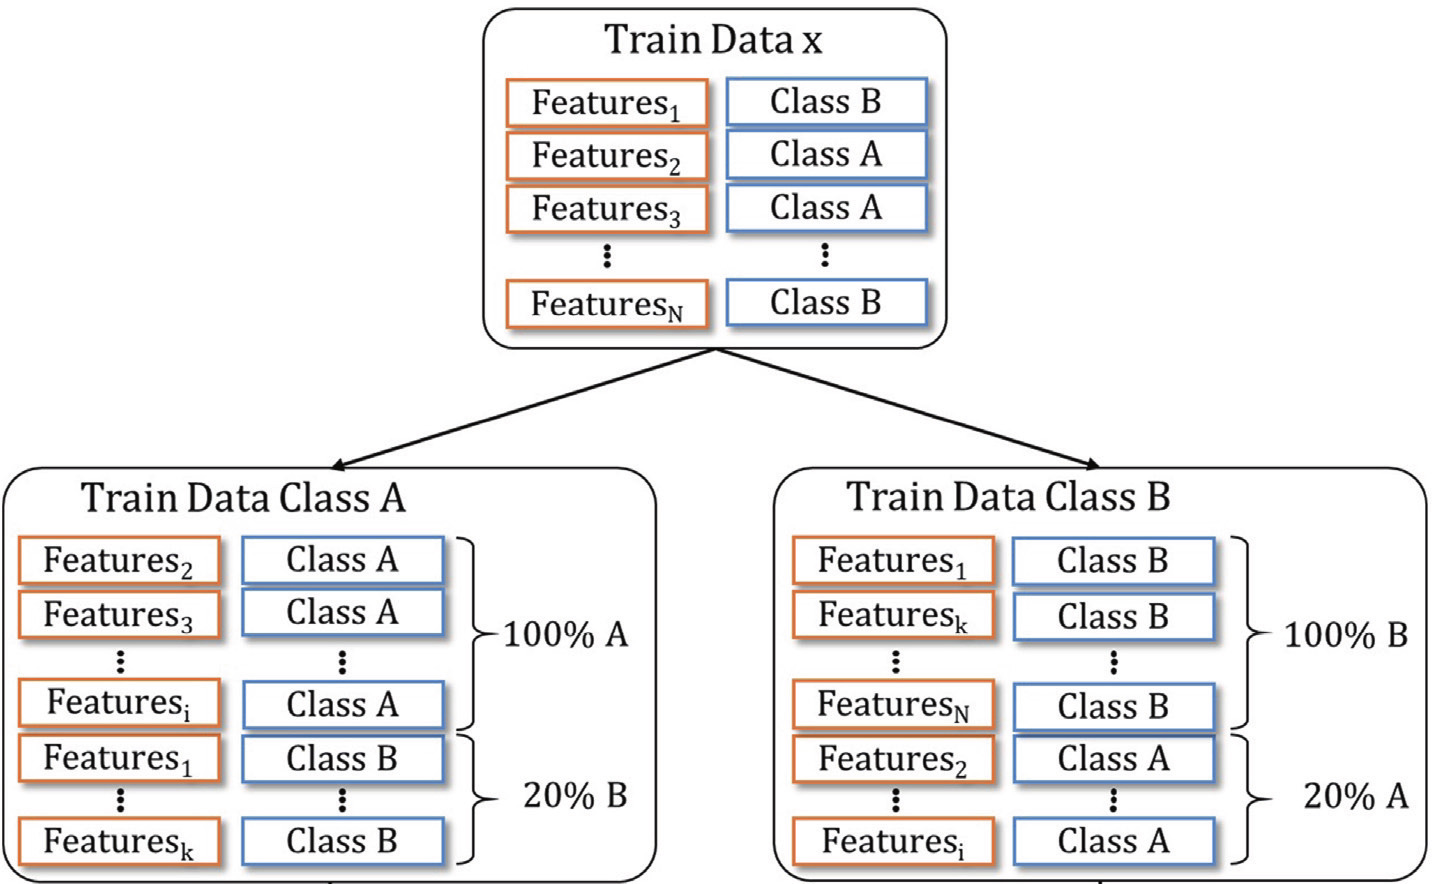
\includegraphics[width=.6\textwidth]{gfx/methodology/ds_split}
  \caption{Die Aufteilung der Datensätze beim Multi-VAE Ansatz. Der vollständige Datensatz wird in klassenweise partitioniert. Zusätzlich wird der Ansatz betrachtet, zu den Daten der Klasse $i$ auch Daten der anderen Klassen beizumischen. Bei mehr als 2 verschiedenen Klassen werden die 20\% zusammen aus zufälligen Beispielen der jeweils anderen Klassen gebildet. Abbildung entnommen aus \cite{Moreno-Barea2020}}
  \label{fig:dataset_parts}
\end{figure}



\section{Generative Classifiers}
Da der VAE darauf trainiert wird, nicht Merkmalsvektoren sondern Latent-Vektoren, welche aus einer Distribution gesampelt werden, zu decodieren, sind die generierten Beispiele häufig unscharf oder entsprechen nicht-interpretierbaren Mischformen zweier Klassen. \cite{Moreno-Barea2020} schlagen daher ein weiteres Neuronales Netz, den "Generative Classifier" (GC), vor, um diese Beispiele zu erkennen und zu verwerfen. Dazu wird zu jedem Eingabebeispiel $x$ eine verrauschte Variante $\tilde{x}$ erzeugt. Das Netzwerk wird auf die binäre Klassifikation von Rauschen und Originalbeispiel trainiert. \cite{Moreno-Barea2020} verwenden Rauschen aus zwei Quellen:
\begin{itemize}
  \item Uniformes Rauschen: Repräsentiert, dass dieses Beispiel "nur Rauschen" beinhaltet
  \item Normalverteiltes Rauschen: Repräsentiert verrauschte Originalbeispiele. Der Erwartungswert der Normalverteilung ist der Sample-Mean über die Originalbeispiele und die Varianz ist ein einstellbarer Hyperparameter $\sigma_{gc}$
\end{itemize}
Mit $\sigma_{gc}$ kann die Sensitivität des Generative Classifiers beeinflusst werden.\\

Da auf Bilddaten die verrauschten Beispiele $\tilde{x}$ nicht den verrauschten Beispielen des VAEs entsprechen, wird in dieser Arbeit eine weitere Art von Trainings Beispielen für den GC vorgeschlagen. Während des VAE Trainings wird eine frühe Version des Modells zwischengespeichert. Diese frühe Modellversion erzeugt in der Regel noch sehr verrauschte Rekonstruktionen. Diese können genutzt werden, um den GC darauf zu trainieren. Diese Art des GC wird auf dem MNIST Datensatz verwendet.

\begin{figure}[hbt]
  \centering
  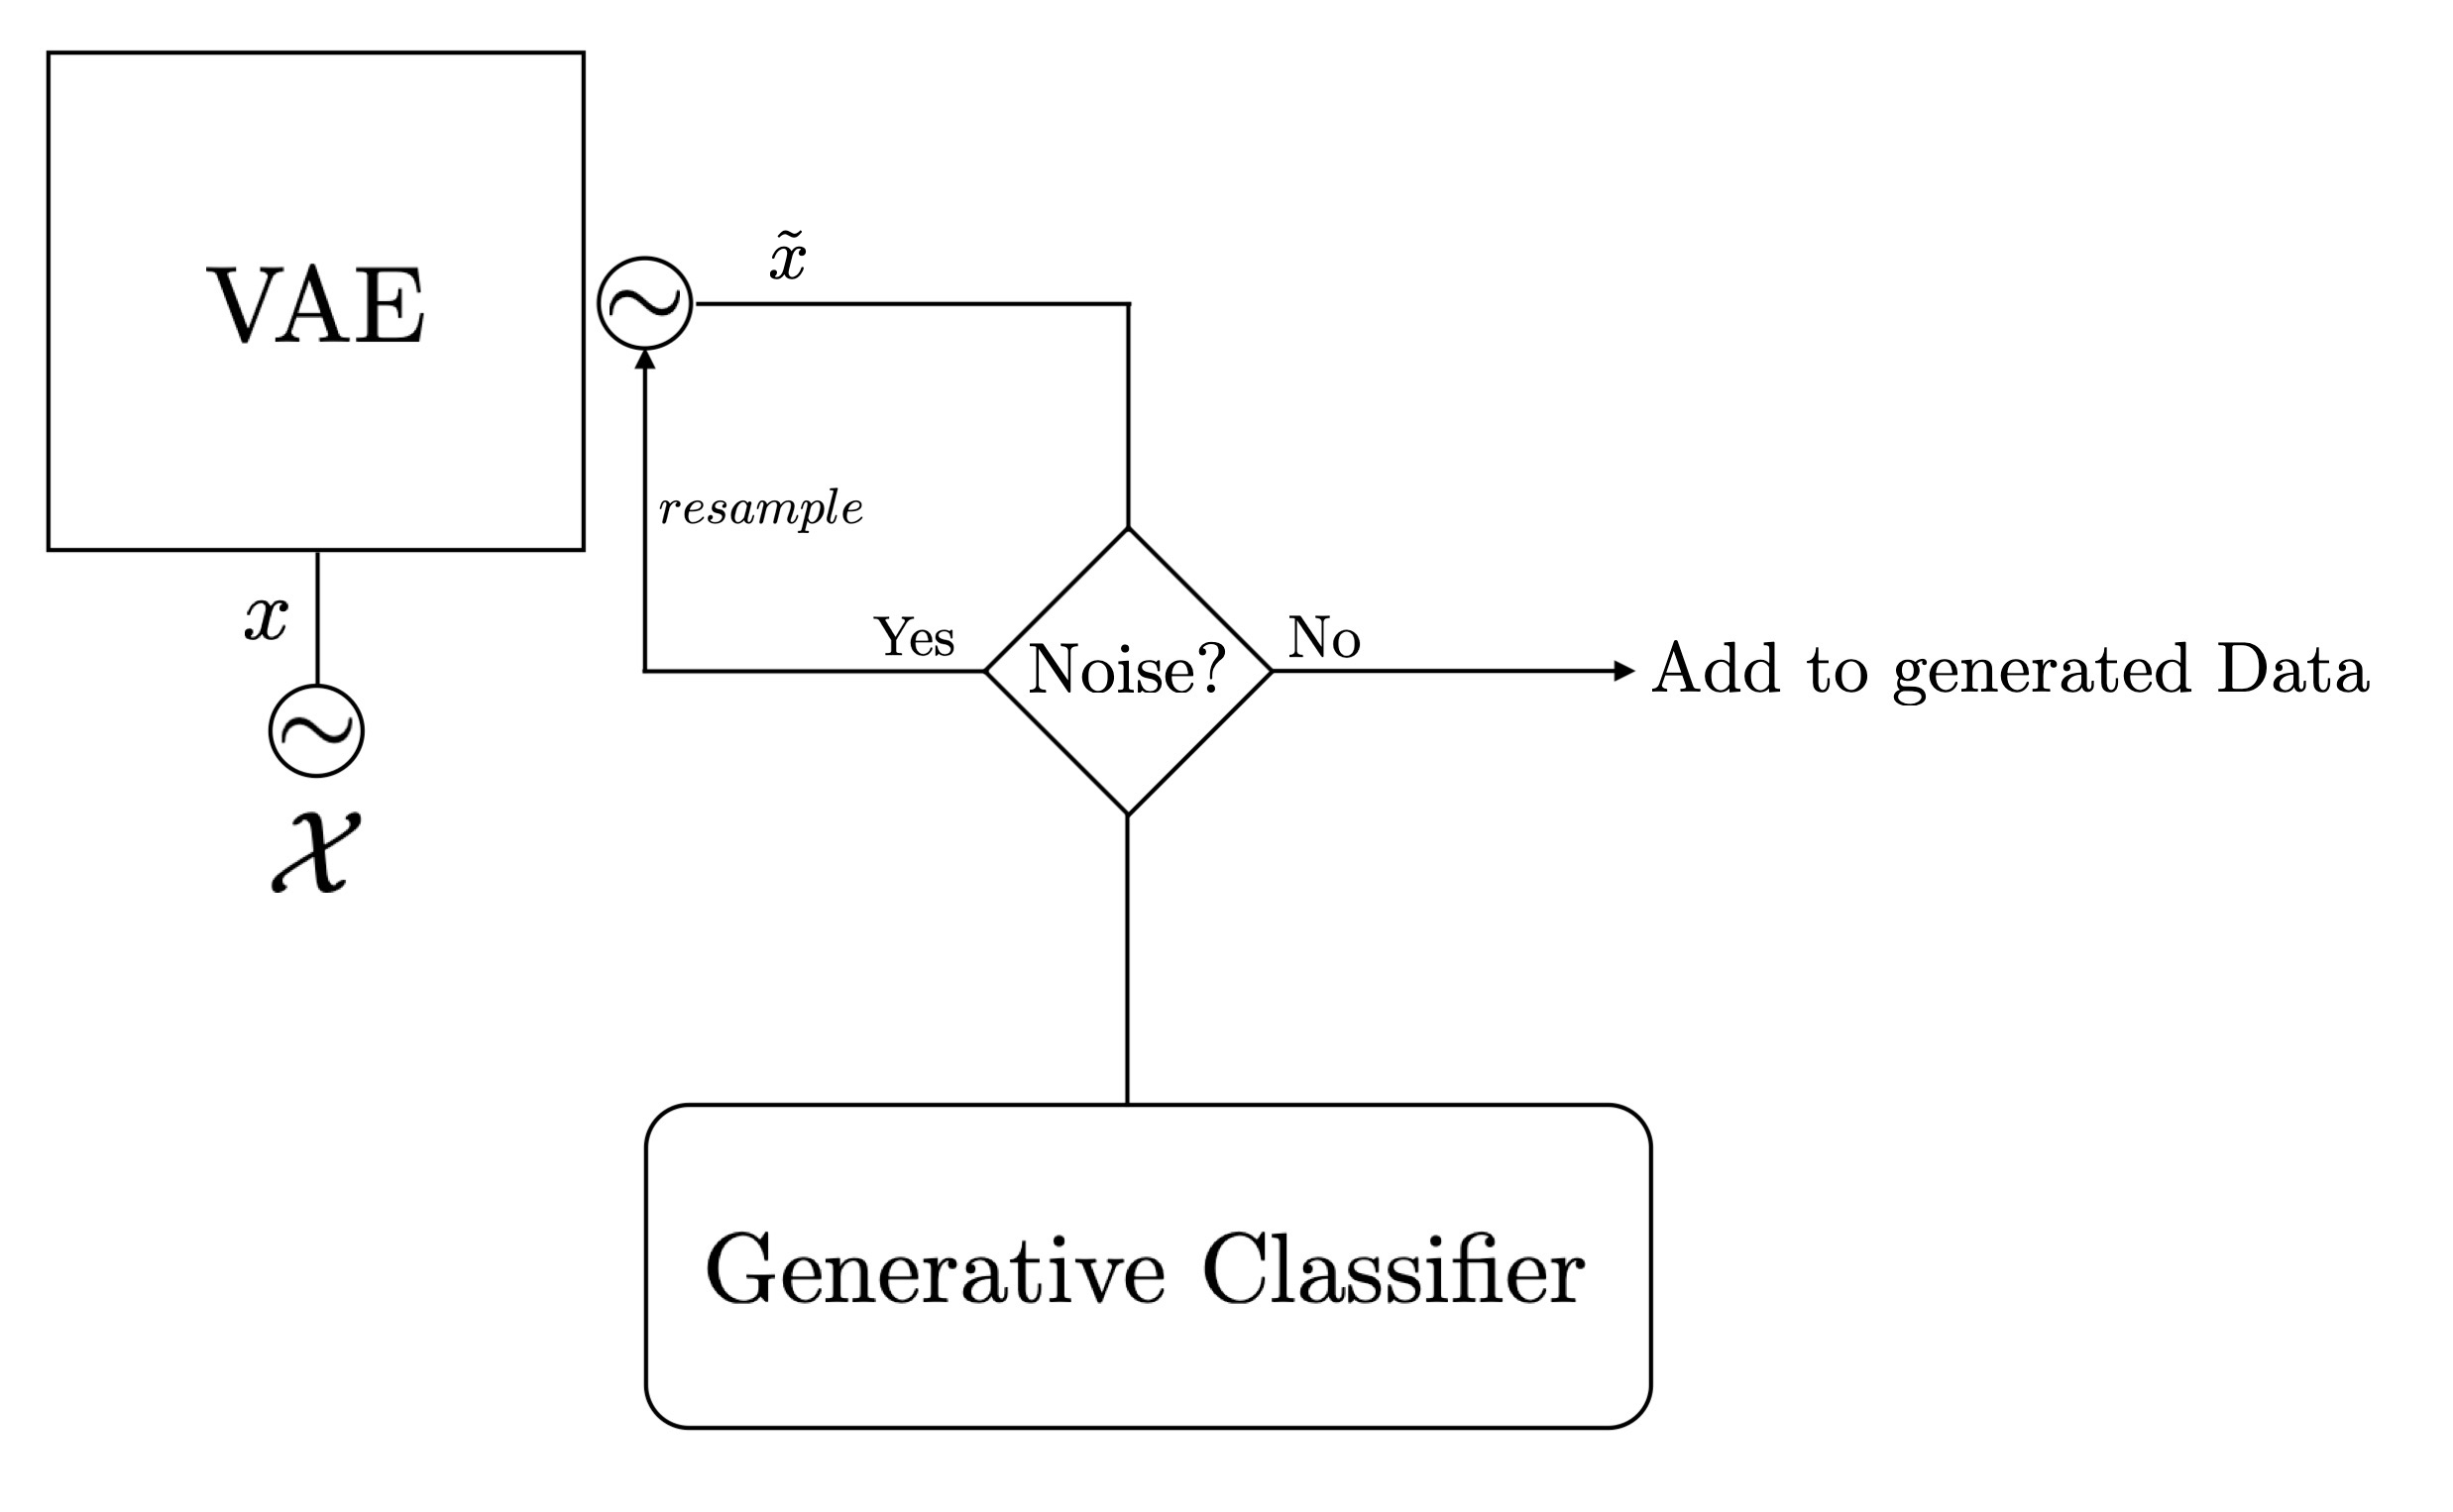
\includegraphics[width=.8\textwidth]{gfx/methodology/gc}
  \caption{Der Generative Classifier dient dazu, verrauschte und verschwommene Daten während des Generations Prozesses auszusortieren. Wenn ein generierter Datenpunkt $\tilde{x}$ als \textit{Noise} klassifiziert wird, erzeugt der VAE ein neues Beispiel.}
\end{figure}



\section{Details zu den VAE Modellarchitekturen}
Wie schon im Abschnitt \ref{sec:VAE_introduction} eingeführt besteht der Variational Autoencoder aus einem Encoder und einem Decoder Teil.
Der Encoder extrahiert Merkmale aus der Eingabe $x$ und bildet diese auf eine $d$-dimensionale Normalverteilung $Q_\phi(z \vert x) = \cN(\mu_\phi(x), \sigma_\phi(x))$ ab. Die Verteilung ist durch die Ausgaben $\mu_\phi(x)$ und $\sigma_\phi(x)$ des Encoders parametrisiert. Man beachte, dass aus numerischen Gründen tatsächlich die logarithmische Varianz $\log \sigma_\phi(x)$ berechnet wird. Das in Abschnitt \ref{sec:reparam_trick} beschriebene Sampling findet nur während des Trainings statt. Für das Generieren neuer Beispiele wurden die in \ref{sec:sampling} erklärten Sampling Methoden genutzt. Wie im Abschnitt \ref{sec:autoencoder} motiviert, wurden auf Bilddaten Konvolutionen für die Merkmalsextraktionen im Encoder verwendet. Der Decoder besteht respektive aus den entsprechenden transponierten Konvolutionen, welche den Latent-Vektor auf Bildgröße hochskalieren. Für die numerischen Daten des Datensatzes PROBEN1 werden keine Konvolutionen verwendet, da die Eingabeattribute dieses Datensatzes eindimensional und unabhängig voneinander sind (vgl. Abschnitt \ref{sec:PROBEN1_dataset}).

Für unsere Experimente wurden die in Tabelle \ref{tab:vae_models} spezifizierten Modell Architekturen gewählt. "Batch-Normalization" wurde zwischen allen Layer genutzt und "LeakyRelu" als Aktivierungsfunktion verwendet, um das Training zu stabilisieren (siehe \cite{Garay-Maestre2019}). Der Log-Likelihood Fehler wird über die "Binary-Cross-Entropy" (BCE) zwischen Eingabe und Rekonstruktion minimiert. Für den KL-Term wurde die in Abschnitt \ref{sec:vae_loss_func} angegebene Formel genutzt. Als Reduktion über die Batches für den Binary-Cross-Entropy Term und die KL-Divergenz wurde "Mean" benutzt, allerdings wird der BCE Term mit der Eingabegröße skaliert, um diesen höher zu gewichten.

\begin{table}[t]
\centering
\scalebox{0.75}{\begin{tabular}{l|l|ll}
\toprule
Datensatz / VAE-Ansatz & Netzwerk & \multicolumn{2}{l}{Konfiguration}                                       \\ \midrule
MNIST Single-VAE       & Encoder  & $Conv(64, 4 \times 4)$           & $Flatten()$                           \\
                       &          & $Conv(128, 4 \times 4)$          & $Linear(128)$                         \\
                       &          & $Conv(256, 4 \times 4)$          & $\mu = Linear(d), \sigma = Linear(d)$ \\ \cline{2-4} 
                       & Decoder  & $Linear(128)$                    & $ConvT(64, 4 \times 4)$               \\
                       &          & $Reshape(256 \times 4 \times 4)$ & $ConvT(1, 4 \times 4)$                \\
                       &          & $ConvT(128, 4 \times 4)$         & $Sigmoid()$                           \\ \midrule
MNIST Multi-VAE        & Encoder  & $Conv(32, 4 \times 4)$           & $Flatten()$                           \\
                       &          & $Conv(64, 4 \times 4)$           & $\mu = Linear(d), \sigma = Linear(d)$ \\ \cline{2-4} 
                       & Decoder  & $Linear(64 \cdot 4 \cdot 4)$     & $ConvT(1, 4 \times 4)$                \\
                       &          & $Reshape(64 \times 4 \times 4)$  & $Sigmoid()$                           \\
                       &          & $ConvT(32, 4 \times 4)$          &                                       \\ \midrule
MNIST Classification   & Classifier & $Conv(8, 5 \times 5)$          & $Flatten()$                           \\
                       &            & $MaxPool2D(2)$                 & $Linear(64)$                          \\
                       &            & $Conv(16, 5 \times 5)$         & $Dropout(0.5)$                        \\
                       &            & $Dropout(0.5)$                 & $Linear(10)$                          \\
                       &            & $MaxPool2D(2)$                 & $LogSoftmax()$                        \\ \midrule
PROBEN1 Multi-VAE      & Encoder  & $Linear(512)$                    & $Linear(64)$                          \\
                       &          & $Linear(256)$                    & $\mu = Linear(d), \sigma = Linear(d)$ \\
                       &          & $Linear(128)$                    &                                       \\ \cline{2-4} 
                       & Decoder  & $Linear(64)$                     & $Linear(512)$                         \\
                       &          & $Linear(128)$                    & $Linear(\text{input\_size})$          \\
                       &          & $Linear(256)$                    & $Sigmoid()$                           \\ \midrule
PROBEN1 Classification & Classifier & $Linear(512)$                  & $Linear(128)$                         \\
                       &            & $Dropout(0.1)$                 & $Dropout(0.1)$                        \\
                       &            & $Linear(256)$                  & $Linear(n\_classes)$                  \\
                       &            & $Dropout(0.1)$                 & $LogSoftmax()$                        \\ \midrule
CIFAR-10 Single-VAE    & Encoder  & $Conv(64, 4 \times 4)$           & $Flatten()$                           \\
                       &          & $Conv(256, 4 \times 4)$          & $Linear(128)$                         \\
                       &          & $Conv(512, 4 \times 4)$          & $\mu = Linear(d), \sigma = Linear(d)$ \\ \cline{2-4} 
                       & Decoder  & $Linear(128)$                    & $ConvT(64, 4 \times 4)$               \\
                       &          & $Reshape(512 \times 4 \times 4)$ & $ConvT(1, 4 \times 4)$                \\
                       &          & $ConvT(256, 4 \times 4)$         & $Sigmoid()$                           \\ \midrule
CelebA-10 Single-VAE   & Encoder  & $Conv(64, 4 \times 4)$           & $Flatten()$                           \\
                       &          & $Conv(128, 4 \times 4)$          & $Linear(128)$                         \\
                       &          & $Conv(256, 4 \times 4)$          & $\mu = Linear(d), \sigma = Linear(d)$ \\
                       &          & $Conv(512, 4 \times 4)$          &                                       \\ \cline{2-4} 
                       & Decoder  & $Linear(128)$                    & $ConvT(64, 4 \times 4)$               \\
                       &          & $Reshape(512 \times 4 \times 4)$ & $ConvT(1, 4 \times 4)$                \\
                       &          & $ConvT(256, 4 \times 4)$         & $Sigmoid()$                           \\
                       &          & $ConvT(128, 4 \times 4)$         &                                       \\
\bottomrule
\end{tabular}}
\caption{Architektur der verwendeten VAE Modelle (spaltenweise angegeben). Mit $Linear(m)$ wird ein "Fully-Connected"-Layer mit $m$ Ausgabe-Features beschrieben. $Conv(m, n \times n)$ bezeichnet eine 2D Konvolution mit Kernelgröße $n \times n$, $ConvT$ analog für 2D transponierte Konvolution. $m$ bezeichnet hierbei die Anzahl an Ausgabe Featuremaps der jeweiligen Konvolution. In allen Konvolutionen wurde Zero-Padding der Größe 1 angewandt, ebenso wie eine Stride von 2. Dies führt zu einer Halbierung der Bildgröße in jedem $Conv$-Layer. Ausnahme stellt das MNIST Klassifikations Netzwerk dar: Hier wurde Stride 2 verwendet und \textit{MaxPooling2D} um eine Dimensionsreduktion zu erreichen. Für die Ausgabelayer $\mu$ und $\sigma$ ist $d$ die Dimension des Latent-Spaces.}
\label{tab:vae_models}
\end{table}


\subsection{Hyperparameter für KL-Divergenz Gewichtung}\label{sec:beta_vae}
\cite{Higgins2017} zeigen empirisch, dass es sinnvoll ist, für das Training des VAE einen Hyperparameter $\beta$ einzuführen. Dieser gewichtet den KL-Term in der Fehlerfunktion und ermöglicht es, einen Trade-Off zwischen einem strukturierten Merkmalsraum und der Qualität der Rekonstruktion zu steuern. Größere Werte lenken den Encoder Output $\mu_\phi(x)$ näher gegen 0. Mit Werten $< 1$ sind die $\mu_\phi(x)$ weniger beschränkt, d.h. Verteilung $\mu[\cX]$ liegt nicht mehr zentral bei 0 und kann beliebige Strukturen annehmen. Da beliebig verteilte Erwartungswerte weniger überlappende Verteilungen zur Folge haben, ermöglicht ein kleinerer Wert für $\beta$ schärfere Rekonstruktionen. \\

Desweiteren geben die Autoren eine Berechnungsvorschrift für ein normalisiertes $\beta$ an, welches die Gewichtung in Abhängigkeit der Dimension der Eingabe $N$ und der Größe des Latent-Spaces kontrolliert.
\begin{equation}
  \beta_{norm} = \beta \cdot \frac{d}{N}, 
\end{equation}
mit Latent-Space Dimension $d$.
